\documentclass[11pt]{standalone}
\usepackage{tikz}
\usetikzlibrary{shapes.geometric}
\usetikzlibrary{arrows.meta,calc,decorations.pathmorphing,shapes.geometric,backgrounds,plotmarks,shapes.multipart}
\begin{document} 
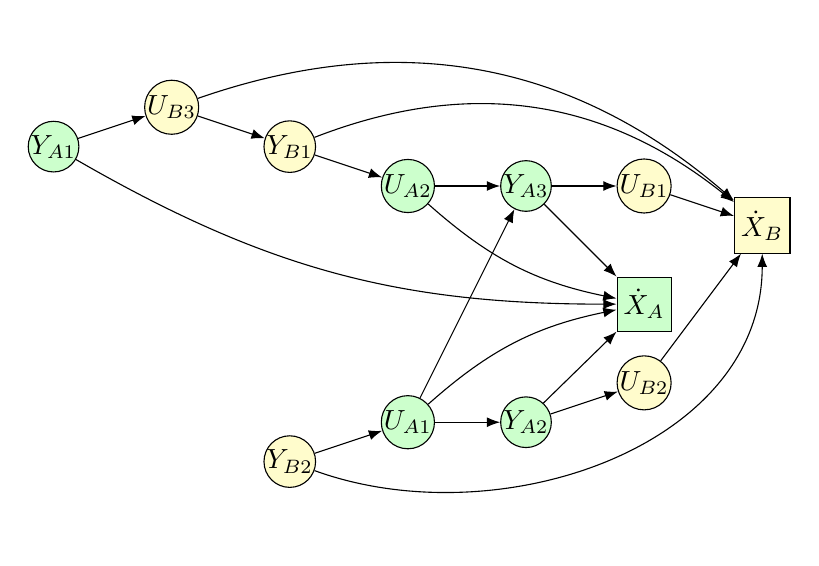
\begin{tikzpicture}[node distance=1.5cm,operation/.style={circle,draw,,inner sep=0},square/.style={draw,regular polygon,regular polygon sides=4,inner sep=-.5}]

% Nodes
\node[operation,fill=green!20] (o5) {$Y_{A1}$};
\node[operation,right of = o5,yshift=.5cm,fill=yellow!20] (o4) {$U_{B3}$};
\node[operation,right of = o4,yshift=-.5cm,fill=yellow!20] (o8) {$Y_{B1}$};
\node[operation,right of = o8,yshift=-.5cm,fill=green!20] (o1) {$U_{A2}$};
\node[operation,right of = o1,fill=green!20] (o7) {$Y_{A3}$};
\node[operation,right of = o7,fill=yellow!20] (o2) {$U_{B1}$};
\node[square,right of = o2,yshift=-.5cm,fill=yellow!20] (o11) {$\dot{X}_{B}$};
\node[square,below of = o2,fill=green!20] (o10) {$\dot{X}_{A}$};
\node[operation,below of = o10,yshift=.5cm,fill=yellow!20] (o3) {$U_{B2}$};
\node[operation,left of = o3,yshift=-.5cm,fill=green!20] (o6) {$Y_{A2}$};
\node[operation,left of = o6,fill=green!20] (o0) {$U_{A1}$};
\node[operation,left of = o0,yshift=-.5cm,fill=yellow!20] (o9) {$Y_{B2}$};

%arcs
\path (o5) edge[-{Latex[]},bend right = 15] (o10);
\path (o5) edge[-{Latex[]}] (o4);
\path (o4) edge[-{Latex[]}] (o8);
\path (o4) edge[-{Latex[]},bend left=30] (o11);
\path (o8) edge[-{Latex[]}] (o1);
\path (o8) edge[-{Latex[]},bend left=30] (o11);
\path (o1) edge[-{Latex[]}] (o7);
\path (o1) edge[-{Latex[]},bend right=15] (o10);
\path (o7) edge[-{Latex[]}] (o2);
\path (o7) edge[-{Latex[]}] (o10);
\path (o2) edge[-{Latex[]}]  (o11);
\path (o9) edge[-{Latex[]}]  (o0);
\path (o9) edge[-{Latex[]}, out=340,in=270]  (o11);
\path (o0) edge[-{Latex[]}]  (o6);
\path (o0) edge[-{Latex[]},bend left=15]  (o10);
\path (o6) edge[-{Latex[]}]  (o3);
\path (o6) edge[-{Latex[]}]  (o10);
\path (o3) edge[-{Latex[]}]  (o11);
\path (o0) edge[-{Latex[]}]  (o7);

\end{tikzpicture}
\end{document}